\begin{center}
	\begin{tabular}{M{10cm}M{8cm}}
		\textbf{TRƯỜNG THCS-THPT NGUYỄN KHUYẾN}& \textbf{ÔN TẬP GIỮA HỌC KÌ 1}\\
		\textbf{MÃ ĐỀ: 002}& \textbf{Bài thi môn: VẬT LÝ 10}\\
		\textit{(Đề thi có 05 trang)}& \textit{Thời gian: 45 phút, không kể phát đề}
		
		\noindent\rule{4cm}{0.8pt} \\
	\end{tabular}
\end{center}
\setcounter{section}{0}
\section{Câu trắc nghiệm nhiều phương án lựa chọn}
\textit{Thí sinh trả lời từ câu 1 đến câu 20. Mỗi câu hỏi thí sinh chọn một phương án}
\setcounter{ex}{0}
\Opensolutionfile{ans}[ans/D10-GKI-002-TN]
% ===================================================================
\begin{ex}
	Điều nào sau đây là \textbf{đúng} khi nói về tốc độ trung bình?
	\choice
	{Tốc độ trung bình là trung bình cộng của các vận tốc}
	{Tốc độ trung bình cho biết tốc độ của vật tại một thời điểm nhất định}
	{Trong hệ SI, đơn vị của tốc độ trung bình là $\si{\meter/\second^2}$}
	{\True Tốc độ trung bình được xác định bằng thương số giữa quãng đường đi được và khoảng thời gian đi hết quãng đường đó}
	\loigiai{}
\end{ex}
% ===================================================================
\begin{ex}
	Hai đại lượng nào sau đây là hai đại lượng vector?
	\choice
	{Quãng đường và tốc độ}
	{\True Độ dịch chuyển và vận tốc}
	{Quãng đường và độ dịch chuyển}
	{Tốc độ và vận tốc}
	\loigiai{}
\end{ex}
% ===================================================================
\begin{ex}
	Chọn phát biểu \textbf{không đúng} về tính chất chuyển động của vật chuyển động thẳng biến đổi đều.
	\choice
	{Vector gia tốc của vật chuyển động thẳng biến đổi đều có phương không đổi}
	{Trong chuyển động nhanh dần đều, gia tốc của vật có độ lớn không đổi theo thời gian và luôn cùng phương, cùng chiều với vector vận tốc của vật}
	{\True Trong chuyển động chậm dần đều, hiệu quãng đường đi được trong những khoảng thời gian liên tiếp luôn không đổi}
	{Đồ thị độ dịch chuyển - thời gian là một nhánh của parabol}
	\loigiai{}
\end{ex}
% ===================================================================
\begin{ex}
	Đại lượng đặc trưng cho tính chất nhanh hay chậm của chuyển động là 
	\choice
	{toạ độ}
	{gia tốc}
	{quãng đường đi}
	{\True tốc độ}
	\loigiai{}
\end{ex}
% ===================================================================
\begin{ex}
	Dựa vào độ dốc của đồ thị vận tốc - thời gian có thể xác định đại lượng nào sau đây?
	\choice
	{Vận tốc}
	{Độ dịch chuyển}
	{Quãng đường}
	{\True Gia tốc}
	\loigiai{}
\end{ex}
% ===================================================================
\begin{ex}
	Khi nhìn vào tốc kế của ô tô đang chạy, số chỉ trên tốc kế cho ta biết
	\choice
	{gia tốc tức thời của ô tô}
	{vận tốc tức thời của ô tô}
	{\True tốc độ tức thời của ô tô}
	{tốc độ trung bình của ô tô}
	\loigiai{}
\end{ex}

% ===================================================================
\begin{ex}
	Công thức tính quãng đường đi được của vật chuyển động thẳng chậm dần đều là
	\choice
	{$x=x_0+v_0t+\dfrac{1}{2}at^2$ ($a$ và $v_0$ cùng dấu)}
	{$x=x_0+v_0t+\dfrac{1}{2}at^2$ ($a$ và $v_0$ trái dấu)}
	{\True $s=v_0t+\dfrac{1}{2}at^2$ ($a$ và $v_0$ trái dấu)}
	{$s=v_0t+\dfrac{1}{2}at^2$ ($a$ và $v_0$ cùng dấu)}
	\loigiai{
		
	}
\end{ex}
% ===================================================================
\begin{ex}
	Trong các đồ thị sau, đồ thị nào là của chuyển động thẳng nhanh dần đều?
	\begin{center}
		\begin{tabular}{M{4cm}M{4cm}M{4cm}M{4cm}}
			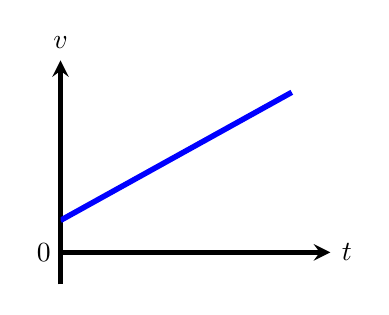
\begin{tikzpicture}  
				\begin{axis}[  ultra thick,scale=0.5,
					xmin=0,  
					xmax=7,  
					ymin=-1,  
					ymax=6, 
					samples=300,
					yticklabels=\empty,
					xticklabels=\empty,
					xtick=\empty,
					ytick=\empty,
					axis lines=center, 
					xlabel=$t$, 		ylabel=$v$,
					every axis y label/.style={at=(current axis.above origin),anchor=south},  
					every axis x label/.style={at=(current axis.right of origin),anchor=west},  ]
					\addplot [line width=2pt, blue, smooth, domain=0:6] {1+2*x/3};  
					\coordinate (O) at (axis cs: 0,0);
				\end{axis}  
				\node[left] at (O) {0};
			\end{tikzpicture}
			&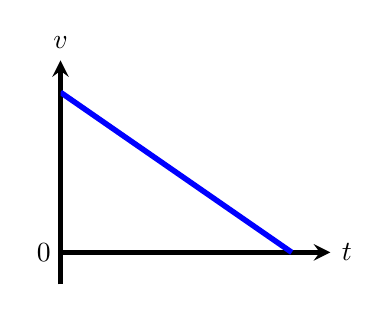
\begin{tikzpicture}  
				\begin{axis}[  ultra thick,scale=0.5,
					xmin=0,  
					xmax=7,  
					ymin=-1,  
					ymax=6, 
					samples=300,
					yticklabels=\empty,
					xticklabels=\empty,
					xtick=\empty,
					ytick=\empty,
					axis lines=center, 
					xlabel=$t$, 		ylabel=$v$,
					every axis y label/.style={at=(current axis.above origin),anchor=south},  
					every axis x label/.style={at=(current axis.right of origin),anchor=west},  ]
					\addplot [line width=2pt, blue, smooth, domain=0:6] {5-5*x/6};  
					\coordinate (O) at (axis cs: 0,0);
				\end{axis}  
				\node[left] at (O) {0};
			\end{tikzpicture}
			&
			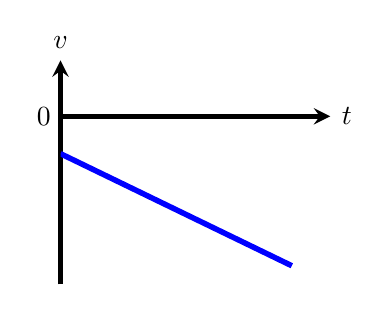
\begin{tikzpicture}  
				\begin{axis}[  ultra thick,scale=0.5,
					xmin=0,  
					xmax=7,  
					ymin=-4.5,  
					ymax=1.5, 
					samples=300,
					yticklabels=\empty,
					xticklabels=\empty,
					xtick=\empty,
					ytick=\empty,
					axis lines=center, 
					xlabel=$t$, 		ylabel=$v$,
					every axis y label/.style={at=(current axis.above origin),anchor=south},  
					every axis x label/.style={at=(current axis.right of origin),anchor=west},  ]
					\addplot [line width=2pt, blue, smooth, domain=0:6] {-1-0.5*x};  
					\coordinate (O) at (axis cs: 0,0);
				\end{axis}  
				\node[left] at (O) {0};
			\end{tikzpicture}
			&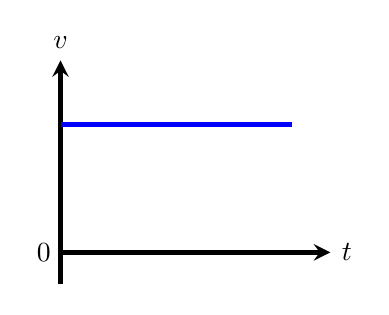
\begin{tikzpicture}  
				\begin{axis}[  ultra thick,scale=0.5,
					xmin=0,  
					xmax=7,  
					ymin=-1,  
					ymax=6, 
					samples=300,
					yticklabels=\empty,
					xticklabels=\empty,
					xtick=\empty,
					ytick=\empty,
					axis lines=center, 
					xlabel=$t$, 		ylabel=$v$,
					every axis y label/.style={at=(current axis.above origin),anchor=south},  
					every axis x label/.style={at=(current axis.right of origin),anchor=west},  ]
					\addplot [line width=2pt, blue, smooth, domain=0:6] {4};  
					\coordinate (O) at (axis cs: 0,0);
				\end{axis}  
				\node[left] at (O) {0};
			\end{tikzpicture}\\
			(I)& (II)& (III)&(IV)
		\end{tabular}
	\end{center}	
	\choice
	{(I), (II) và (III)}
	{(I) và (II)}
	{(I), (II) và (IV)}
	{\True (I) và (III)}
	\loigiai{}
\end{ex}
% ===================================================================
\begin{ex}
	Một chất điểm chuyển động biến đổi với công thức vận tốc $v=4+3t\ \left(\si{\meter/\second}; \si{\second}\right)$. Nhận định nào sau đây là đúng khi nói về chuyển động của chất điểm?	
	\choice
	{Chất điểm chuyển động nhanh dần đều theo chiều dương với gia tốc $\SI{6}{\meter/\second^2}$}
	{Chất điểm chuyển động chậm dần đều theo chiều dương với gia tốc $\SI{3}{\meter/\second^2}$}
	{Chất điểm chuyển động nhanh dần đều theo chiều dương với gia tốc $\SI{4}{\meter/\second^2}$}
	{\True Chất điểm chuyển động nhanh dần đều theo chiều dương với gia tốc $\SI{3}{\meter/\second^2}$}
	\loigiai{}
\end{ex}
% ===================================================================
\begin{ex}
	\immini{
		Hình bên là đồ thị độ dịch chuyển - thời gian của ô tô chuyển động thẳng theo một hướng xác định. Tốc độ lớn nhất của ô tô tương ứng với đoạn nào trên đồ thị?
	}	
	{\includegraphics[width=0.35\linewidth]{../figs/D10-2-11}}
	\choice
	{1}
	{2}
	{\True 3}
	{4}
	\loigiai{}
\end{ex}
% ===================================================================
\begin{ex}
	Hình sau thể hiện giờ đi từ Hà Nội (02/01/2024) và giờ đến Vinh của các tàu SE7, SE5, SE3, SE19.
	\begin{center}
		\includegraphics[width=0.7\linewidth]{../figs/D10-2-12}
	\end{center}
	Trong các tàu nói trên, tàu có tốc độ trung bình lớn nhất là
	\choice
	{\True SE3}
	{SE5}
	{SE7}
	{SE19}
	\loigiai{}
\end{ex}
% ===================================================================
\begin{ex}
	Một mặt bàn hình chữ nhật ABCD có chiều dài $\mathrm{AB}=\SI{0.8}{\meter}$ và chiều rộng $\mathrm{BC}=\SI{0.6}{\meter}$. Một con nhện bò dọc theo các cạnh của mặt bàn, từ A đến C. Độ dịch chuyển của con nhện là
	\choice
	{\True $\SI{1.0}{\meter}$}
	{$\SI{1.4}{\meter}$}
	{$\SI{0.2}{\meter}$}
	{$\SI{1.2}{\meter}$}
	\loigiai{}
\end{ex}
% ===================================================================
\begin{ex}
	Một xe xuất phát từ lúc 7 giờ 15 phút sáng từ thành phố M, chuyển động thẳng đều tới thành phố N, cách thành phố M $\SI{90}{\kilo\meter}$. Biết tốc độ của xe là $\SI{60}{\kilo\meter/\hour}$, xe đến thành phố N lúc	
	\choice
	{9 giờ 45 phút}
	{8 giờ 30 phút}
	{9 giờ 30 phút}
	{\True 8 giờ 45 phút}
	\loigiai{
		Thời gian để xe đi từ M đến N:
		$$\Delta t=\dfrac{s}{v}=\SI{1.5}{\hour}.$$
		Thời điểm xe đến N:
		$$t=\SI{7}{\hour}\SI{15}{\minute}+\Delta t=\SI{8}{\hour}\SI{45}{\minute}.$$	
	}
\end{ex}

% ===================================================================
\begin{ex}
	Một ô tô chạy trên đoạn đường thẳng từ A đến B mất khoảng thời gian $t$. Trong 1/4 đầu của khoảng thời gian $t$ này, ô tô có tốc độ là $\SI{40}{\kilo\meter/\hour}$. Trong khoảng thời gian còn lại, ô tô có tốc độ là $\SI{60}{\kilo\meter/\hour}$. Tốc độ trung bình của ô tô trên cả đoạn đường AB là	
	\choice
	{$\SI{45}{\kilo\meter/\hour}$}
	{$\SI{49}{\kilo\meter/\hour}$}
	{\True $\SI{55}{\kilo\meter/\hour}$}
	{$\SI{50}{\kilo\meter/\hour}$}
	\loigiai{}
\end{ex}
% ===================================================================
\begin{ex}
	Một chiếc thuyền xuôi dòng từ A đến B với tốc độ $\SI{34}{\kilo\meter/\hour}$ đối với nước. Nước chảy với tốc độ $\SI{2}{\kilo\meter/\hour}$ so với bờ sông. Biết hai bến sông cách nhau $\SI{120}{\kilo\meter}$. Thời gian thuyền đi từ A đến B là
	\choice
	{$\SI{2.94}{\hour}$}
	{$\SI{4.26}{\hour}$}
	{\True $\SI{3.33}{\hour}$}
	{$\SI{2.63}{\hour}$}
	\loigiai{
		Thời gian xuôi dòng:
		$$t_{\text{xd}}=\dfrac{s}{v_t+v_n}\approx\SI{3.33}{\hour}.$$
	}
\end{ex}
% ===================================================================
\begin{ex}
	Một người bơi dọc theo chiều dài $\SI{55}{\meter}$ của bể bơi hết $\SI{50}{\second}$ rồi quay về lại chỗ xuất phát trong $\SI{60}{\second}$. Trong suốt quãng đường đi và về vận tốc trung bình của người đó là
	\choice
	{\True $\SI{0}{\meter/\second}$}
	{$\SI{1.0}{\meter/\second}$}
	{$\SI{1.1}{\meter/\second}$}
	{$\SI{2.0}{\meter/\second}$}
	\loigiai{
		Vì điểm đầu của quĩ đạo chuyển động trùng với điểm cuối nên $d=0\Rightarrow v=0$.	
	}
\end{ex}
% ===================================================================
\begin{ex}
	Xe ô tô đang chuyển động thẳng với vận tốc $\SI{20}{\meter/\second}$ thì hãm phanh chuyển động chậm dần đều. Quãng đường xe đi được từ lúc hãm phanh đến khi xe dừng hẳn là $\SI{100}{\meter}$. Gia tốc của xe là
	\choice
	{$\SI{1}{\meter/\second^2}$}
	{$\SI{5}{\meter/\second^2}$}
	{\True $\SI{-2}{\meter/\second^2}$}
	{$\SI{-1}{\meter/\second^2}$}
	\loigiai{}
\end{ex}
% ===================================================================
\begin{ex}
	Công thức độ dịch chuyển của một vật là $d=-3t+2t^2$ ($x$ tính bằng mét, $t$ tính bằng giây). Công thức vận tốc của vật là
	\choice
	{$v=-3+2t$}
	{\True $v=-3+4t$}
	{$v=-3t+2$}
	{$v=3t$}
	\loigiai{}
\end{ex}
% ===================================================================
\begin{ex}
	Hình bên là đồ thị toạ độ - thời gian của một chiếc xe máy đang chạy trên đường thẳng. Xe này có tốc độ là
	\begin{center}
		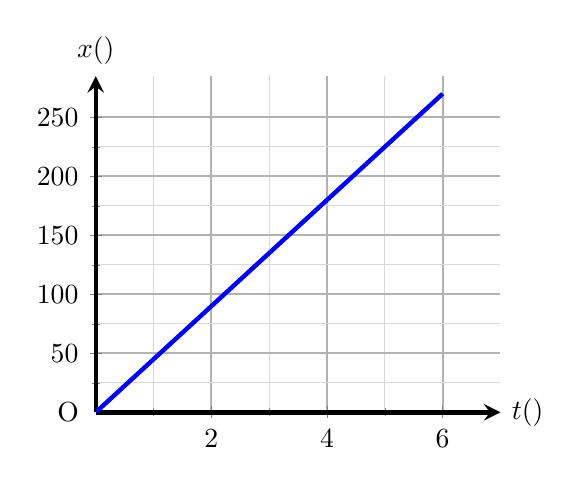
\begin{tikzpicture}  
			\begin{axis}[  ultra thick,scale=0.75,
				xmin=0,  
				xmax=7,  
				xtick={0,2,...,6},
				ytick={0,50,...,250},
				minor x tick num=1,
				minor y tick num=1,
				ymin=0,  
				ymax=285, 
				samples=300,
				axis lines=center, 
				grid style={step=1, line width =0.4pt, color=gray!30!white},
				grid=both, %giới hạn ô lưới
				major grid style={line width=0.8pt,gray!60!white},
				xlabel=$\xsi{t}{\left(\si{\hour}\right)}$, 		ylabel=$\xsi{x}{\left(\si{\kilo\meter}\right)}$,
				every axis y label/.style={at=(current axis.above origin),anchor=south},  
				every axis x label/.style={at=(current axis.right of origin),anchor=west},  ] 
				\addplot [ultra thick, blue, smooth, domain=0:6] {45*x}; 
			\end{axis} 
			\node at (-0.35,0) {O}; 
		\end{tikzpicture}
		
	\end{center}
	\choice
	{\True $\SI{45}{\kilo\meter/\hour}$}
	{$\SI{43.75}{\kilo\meter/\hour}$}
	{$\SI{45.45}{\kilo\meter/\hour}$}
	{$\SI{50}{\kilo\meter/\hour}$}
	\loigiai{
		Tại $t=\SI{5}{\hour}$ thì $x=\SI{225}{\kilo\meter}$:
		$$\left|v\right|=\left|\dfrac{\Delta x}{\Delta t}\right|=\SI{45}{\kilo\meter/\hour}.$$	
	}
\end{ex}

% ===================================================================
\begin{ex}
	Một ô tô đang chạy với tốc độ $\SI{72}{\kilo\meter/\hour}$ thì hãm phanh chuyển động thẳng chậm dần đều với gia tốc có độ lớn $\SI{0.5}{\meter/\second^2}$. Quãng đường mà ô tô đã đi được trong 5 giây cuối trước khi dừng lại là
	\choice
	{$\SI{68.75}{\meter}$}
	{$\SI{81.25}{\meter}$}
	{$\SI{12.5}{\meter}$}
	{\True $\SI{6.25}{\meter}$}
	\loigiai{
		Đảo ngược thời gian sẽ thấy xe chuyển động nhanh dần đều với gia tốc $a=\SI{0.5}{\meter/\second^2}$, không vận tốc đầu. Lúc này, 5 giây cuối trở thành 5 giây đầu:
		$$s=\dfrac{1}{2}at^2=\dfrac{1}{2}\cdot0,5\cdot5^2=\SI{6.25}{\meter}.$$
	}
\end{ex}

\Closesolutionfile{ans}
\section{Câu trắc nghiệm đúng/sai} 
\textit{Thí sinh trả lời từ câu 1 đến câu 2. Trong mỗi ý \textbf{a)}, \textbf{b)}, \textbf{c)}, \textbf{d)} ở mỗi câu, thí sinh chọn đúng hoặc sai}
\setcounter{ex}{0}
\Opensolutionfile{ans}[ans/D10-GKI-002-TF]
\begin{ex}
	Một vật chuyển động thẳng có đồ thị vận tốc theo thời gian như hình bên dưới.
	\begin{center}
		\includegraphics[width=0.7\linewidth]{../figs/D10-2-8}
	\end{center}
	\choiceTF[t]
	{Vật đạt tốc độ lớn nhất tại B}
	{Trong quá trình AB, vật chuyển động thẳng đều}
	{Trong quá trình EF, vật đứng yên}
	{\True Độ lớn gia tốc tại D lớn hơn độ lớn gia tốc tại B}
	\loigiai{
		\begin{itemchoice}
			\itemch Sai. Vật đạt tốc độ lớn nhất tại C.
			\itemch Sai. Trong quá trình AB, vật chuyển động biến đổi.
			\itemch Sai. Trong quá trình EF, tốc độ của vật khác 0.
			\itemch Đúng. Độ dốc đồ thị tại D lớn hơn độ dốc của đồ thị tại B. 
		\end{itemchoice}
	}
\end{ex}

% ===================================================================
\begin{ex}
	Một thiết bị tạo ra các chấm trên một băng giấy chuyển động với khoảng thời gian giữa 2 chấm liên tiếp là $\SI{0.02}{\second}$. Hình 1, Hình 2 và Hình 3 biểu diễn kết 3 quả chuyển động thẳng của băng giấy. Mốc thời gian được chọn tại chấm 0.
	\begin{center}
		\includegraphics[width=0.4\linewidth]{../figs/D10-2-9}
	\end{center}
	\choiceTF[t]
	{\True Kết quả ở Hình 1 chứng tỏ băng giấy chuyển động thẳng đều}
	{Kết quả ở Hình 2 và Hình 3 chứng tỏ băng giấy chuyển động nhanh dần}
	{\True Tốc độ trung bình của băng giấy ở Hình 1 và Hình 2 trong $\SI{0.1}{\second}$ (tính từ mốc thời gian) là bằng nhau}
	{Độ lớn gia tốc của băng giấy ở Hình 2 lớn hơn độ lớn gia tốc của băng giấy ở Hình 3}
	\loigiai{
		\begin{itemchoice}
			\itemch Đúng.
			\itemch Sai. Hình 2 băng giấy chuyển động nhanh dần, Hình 3 băng giấy chuyển động chậm dần.
			\itemch Đúng.
			\itemch Sai. Chưa thể khẳng định vật chuyển động biến đổi đều nên chưa thể so sánh gia tốc trong 2 trường hợp.
		\end{itemchoice}
	}
\end{ex}
\Closesolutionfile{ans}
\section{Câu trắc nghiệm trả lời ngắn} \textit{Thí sinh trả lời từ câu 1 đến câu 6}
\setcounter{ex}{0}
\Opensolutionfile{ans}[ans/D10-GKI-002-TL]
% ===============================================================
\begin{ex}
	\immini{
		Chuyển động của một viên bi có đồ thị vận tốc - thời gian như hình bên. Ở thời điểm nào (tính bằng giây), vận tốc viên bi có giá trị bằng không?
	}
	{\vspace{-0.5cm}\includegraphics[scale=0.7]{../figs/D10-2-13}}
	\shortans{2 }
	\loigiai{
		
	}
\end{ex}
% ===================================================================
\begin{ex}
	Một con bọ rùa bò đều trên các cạnh của một tấm ván hình chữ nhật với chiều dài các cạnh $\mathrm{AB}=\SI{40}{\centi\meter}$, $\mathrm{BC}=\SI{20}{\centi\meter}$, mỗi 2 giây nó bò được $\SI{1.5}{\centi\meter}$. Tại thời điểm ban đầu, con bọ rùa ở đỉnh A của tấm ván. Kể từ thời điểm ban đầu, trong thời gian $\SI{80}{\second}$, vận tốc trung bình là bao nhiêu $\si{\centi\meter/\second}$? \textit{(Kết quả làm tròn đến 2 chữ số sau dấu thập phân.)}
	\shortans{$0,56$}
	\loigiai{
		Trong $\SI{80}{\second}$ con bọ rùa bò được $\SI{60}{\centi\meter}$ nên đi được hết cạnh AC và BC.\\
		$$v=\dfrac{\sqrt{\mathrm{AC}^2+\mathrm{BC}^2}}{t}\approx\SI{0.56}{\centi\meter/\second}.$$
	}
\end{ex}
% ===================================================================
\begin{ex}
\immini{	Chuyển động của hai viên bi $\mathrm{B}_1$ và $\mathrm{B}_2$ có đồ thị vận tốc thời gian như hình bên. Gọi $s_1$ và $s_2$ là quãng đường đi được tương ứng của $\mathrm{B}_1$ và $\mathrm{B}_2$ trong cùng thời gian kể từ thời điểm $t=\SI{0}{\second}$. Tỉ số $s_2/s_1$ là bao nhiêu? \textit{(Kết quả lấy đến 1 chữ số sau dấu phẩy thập phân)}.}
{\begin{tikzpicture} 
		\coordinate (O)  at (0,0);
		\coordinate (t) at (4,0);
		\coordinate (v) at (0,4);
		\coordinate (A) at ($(O)+(30:3)$);
		\coordinate (B) at ($(O)+(60:3.5)$);
		\draw[line width=1pt, -latex] (O)--(v);
		\draw[line width=1pt, -latex] (O)--(t);
		\draw[line width=1.5pt, red] (O)--(A);
		\draw[line width=1.5pt, blue] (O)--(B);
		\node[left] at (O) {O};
		\node[above] at (t) {$t$};
		\node[left] at (v) {$v$};
		\tkzFillAngle[size=0.75cm,color=red, fill=red, opacity=0.25](t,O,A);
		\tkzLabelAngle[color=red,pos=1.2](t,O,A){$\SI{30}{\degree}$}
		\tkzMarkAngle[size=0.5cm,color=blue](t,O,B);
		\node[blue] at (0.75,0.7) {$\SI{60}{\degree}$};
		\node[above right, red] at (A) {$\mathrm{B}_2$};
		\node[above right, blue] at (B) {$\mathrm{B}_1$};
\end{tikzpicture}}
	\shortans{0,3}
	\loigiai{
		$$\dfrac{s_2}{s_1}=\dfrac{\dfrac{1}{2}a_2t^2}{\dfrac{1}{2}a_1t^2}=\dfrac{a_2}{a_1}=\dfrac{\tan\SI{30}{\degree}}{\tan\SI{60}{\degree}}\approx0,3.$$
	}
\end{ex}
% ===============================================================
\begin{ex}
	Hình bên dưới mô tả vị trí của xe ô tô trong khoảng thời gian $\SI{5}{\second}$ kể từ lúc xe bắt đầu tăng tốc đều từ trạng thái nghỉ. Sau $\SI{6}{\second}$ xe cách vị trí ban đầu bao nhiêu mét?
	\begin{center}
		\includegraphics[width=0.8\linewidth]{../figs/D10-2-14}
	\end{center}
	\shortans{72}
	\loigiai{
		$$\dfrac{s_6}{s_5}=\dfrac{\dfrac{1}{2}a\cdot6^2}{\dfrac{1}{2}a\cdot5^2}=\dfrac{36}{25}\Rightarrow s_6=50\cdot\dfrac{36}{25}=\SI{72}{\meter}.$$
	}
\end{ex}
% ===============================================================
\begin{ex}
	Trên quãng đường AB có hai xe chuyển động thẳng. Xe 1 đi từ A tới B với tốc độ trung bình $\SI{32}{\kilo\meter/\hour}$. Xe 2 đi từ B đến A, nửa quãng đường đầu chuyển động đều với tốc độ $\SI{60}{\kilo\meter/\hour}$, nửa quãng đường sau chuyển động đều với tốc độ $\SI{40}{\kilo\meter/\hour}$. Hai xe đến đích cùng lúc, xe 1 xuất phát sớm hơn xe 2 một khoảng thời gian 1 giờ. Tính quãng đường AB theo đơn vị kilomet?
	\shortans{96 }
	\loigiai{
		Tốc độ trung bình của xe 2 trên cả đoạn đường BA:
		$$v_{\mathrm{tb2}}=\dfrac{2s}{\dfrac{s}{v_1}+\dfrac{s}{v_2}}=\dfrac{2}{\dfrac{1}{v_1}+\dfrac{1}{v_2}}=\dfrac{2}{\dfrac{1}{60}+\dfrac{1}{40}}=\SI{48}{\kilo\meter/\hour}.$$
		Hai xe đến đích cùng lúc, xe 1 xuất phát sớm hơn xe 2 một khoảng thời gian 1 giờ nên:
		\begin{eqnarray*}
			&&t_1=t_2+1\\
			&\Rightarrow&\dfrac{s}{v_{\mathrm{tb2}}}=\dfrac{s}{v_{\mathrm{tb1}}}+1\\
			&\Leftrightarrow& \dfrac{s}{32}=\dfrac{s}{48}+1\\
			&\Rightarrow& s=\SI{96}{\kilo\meter/\hour}
		\end{eqnarray*}
	}
\end{ex}
% ===============================================================
\begin{ex}
	Hai chất điểm chuyển động trên hai trục tọa độ vuông góc $Ox$, $Oy$ và đi qua $O$ cùng lúc. Vật thứ nhất chuyển động trên trục $Ox$ theo chiều dương với gia tốc không đổi bằng $\SI{1}{\meter/\second^2}$ và tốc độ khi đi qua O là $\SI{6}{\meter/\second}$. Vật thứ hai chuyển động chậm dần đều theo chiều âm trên trục $Oy$ với gia tốc có độ lớn $\SI{2}{\meter/\second^2}$ và  tốc độ khi đi qua O là $\SI{8}{\meter/\second}$. Độ lớn vận tốc nhỏ nhất của vật thứ nhất đối với vật thứ hai trong khoảng thời gian kể từ lúc đi qua O cho đến khi vật thứ hai dừng là bao nhiêu $\si{\meter/\second}$? \textit{(Kết quả làm tròn đến 2 chữ số sau dấu phẩy thập phân)}.
	\shortans{$8,94$}
	\loigiai{
		\begin{center}
			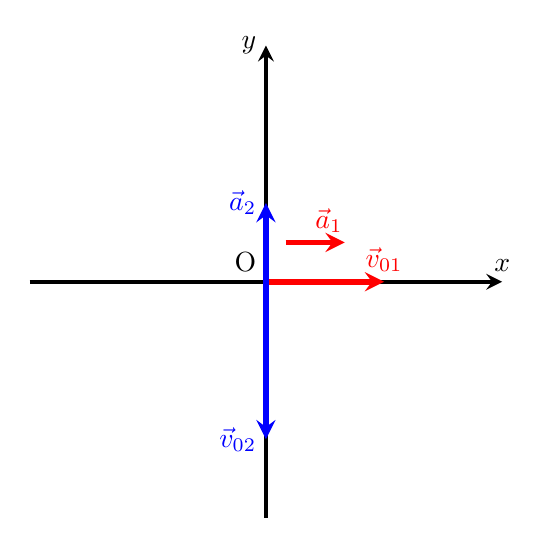
\begin{tikzpicture}
				\coordinate (O) at (0,0);
				\coordinate (x) at (3,0);
				\coordinate (y) at (0,3);
				\coordinate (vx) at (1.5,0);
				\coordinate (vy) at (0,-2);
				\draw[-stealth, line width=1.5pt] (-3,0)--(x);
				\draw[-stealth, line width=1.5pt] (0,-3)--(y);
				\draw[-stealth, line width=2pt, red] (O)--(vx);
				\draw[-stealth, line width=2pt, blue] (O)--(vy);
				\draw[-stealth, line width=2pt, red] (0.25,0.5)--(1,0.5);
				\draw[-stealth, line width=2pt, blue] (O)--(0,1);
				\node[above, red] at (vx) {$\vec{v}_{01}$};
				\node[left, blue] at (vy) {$\vec{v}_{02}$};
				\node[above left] at (O) {O};
				\node[left, blue] at (0,1) {$\vec{a}_2$};
				\node[above, red] at (0.8,0.5) {$\vec{a}_1$};
				\node[above] at (x) {$x$};
				\node[left] at (y) {$y$};
			\end{tikzpicture}
		\end{center}
		Chọn gốc thời gian lúc 2 vật đi qua gốc tọa độ.\\
		Phương trình vận tốc của mỗi vật:
		$$\begin{cases}
			v_1=v_{01}+a_1t\\
			v_2=v_{02}+a_2t
		\end{cases}\Rightarrow\begin{cases}
			v_1=6+t\\
			v_2=8-2t
		\end{cases}.$$
		Vận tốc tương đối của vật thứ nhất đối với vật thứ hai:
		$$\vec{v}_{12}=\vec{v}_1-\vec{v}_2.$$
		Vì $\vec{v}_1\bot\vec{v}_2$ nên:
		\begin{equation}
			\label{eq:1}
			v^2_{12}=v^2_1+v^2_2=5t^2-20t+100
		\end{equation}
		Từ phương trình  \eqref{eq:1}, suy ra giá trị cực tiểu của $v^2_{12}$ là $v^2_{12\min}=80\Rightarrow v_{12\min}=\sqrt{80}\approx\SI{8.94}{\meter/\second}.$
	}
\end{ex}
\Closesolutionfile{ans}
\begin{center}
	\textbf{-- HẾT --}
\end{center}
\newpage
\setcounter{section}{0}
\begin{center}
	\textbf{\large BẢNG ĐÁP ÁN}
\end{center}
\section{}
\inputansbox{10}{ans/D10-GKI-002-TN}
\section{}
\inputansbox[2]{2}{ans/D10-GKI-002-TF}
\section{}
\inputansbox[3]{6}{ans/D10-GKI-002-TL}